% THIS IS AN EXAMPLE DOCUMENT FOR VLDB 2010
% based on ACM SIGPROC-SP.TEX VERSION 2.7
% Modified by  Gerald Weber <gerald@cs.auckland.ac.nz>


% This example *does* use the .bib file (from which the .bbl file
% is produced). REMEMBER HOWEVER: After having produced the .bbl file,
% and prior to final submission, you need to 'insert'  your .bbl file into
% your source .tex file so as to provide ONE 'self-contained' source file.

\documentclass{vldb}
\usepackage{graphicx}
\usepackage{balance}  % for  \balance command ON LAST PAGE  (only there!)


\begin{document}

% ****************** TITLE ****************************************

\title{Using Deep Learning to Perform Fuzzy Joins}

% possible, but not really needed or used for PVLDB:
%\subtitle{[Extended Abstract]
%\titlenote{A full version of this paper is available as\textit{Author's Guide to Preparing ACM SIG Proceedings Using \LaTeX$2_\epsilon$\ and BibTeX} at \texttt{www.acm.org/eaddress.htm}}}

% ****************** AUTHORS **************************************

% You need the command \numberofauthors to handle the 'placement
% and alignment' of the authors beneath the title.
%
% For aesthetic reasons, we recommend 'three authors at a time'
% i.e. three 'name/affiliation blocks' be placed beneath the title.
%
% NOTE: You are NOT restricted in how many 'rows' of
% "name/affiliations" may appear. We just ask that you restrict
% the number of 'columns' to three.
%
% Because of the available 'opening page real-estate'
% we ask you to refrain from putting more than six authors
% (two rows with three columns) beneath the article title.
% More than six makes the first-page appear very cluttered indeed.
%
% Use the \alignauthor commands to handle the names
% and affiliations for an 'aesthetic maximum' of six authors.
% Add names, affiliations, addresses for
% the seventh etc. author(s) as the argument for the
% \additionalauthors command.
% These 'additional authors' will be output/set for you
% without further effort on your part as the last section in
% the body of your article BEFORE References or any Appendices.

\numberofauthors{3} %  in this sample file, there are a *total*
% of EIGHT authors. SIX appear on the 'first-page' (for formatting
% reasons) and the remaining two appear in the \additionalauthors section.

\author{
% You can go ahead and credit any number of authors here,
% e.g. one 'row of three' or two rows (consisting of one row of three
% and a second row of one, two or three).
%
% The command \alignauthor (no curly braces needed) should
% precede each author name, affiliation/snail-mail address and
% e-mail address. Additionally, tag each line of
% affiliation/address with \affaddr, and tag the
% e-mail address with \email.
%
% 1st. author
\alignauthor Abraham Judah Gale \\
% \titlenote{Dr.~Trovato insisted his name be first.}\\
       \affaddr{Thesis Submitted to}\\
       \affaddr{Yeshiva University}\\
  %     \affaddr{Wallamaloo, New Zealand}\\
       \email{yehuda.gale@gmail.com}
% 2nd. author
\alignauthor
Kavitha Srinivas \\
% \titlenote{The secretary disavows
% any knowledge of this author's actions.}\\
     \affaddr{Advisor}\\
       \affaddr{Rivet Labs}\\
 %      \affaddr{Dublin, Ohio 43017-6221}\\
       \email{Kavitha@rivetlabs.io}
% 3rd. author
\alignauthor Judah Diament\\
       \affaddr{Advisor}\\
       \affaddr{Yeshiva University }\\
       \email{diament@yu.edu}
}
% There's nothing stopping you putting the seventh, eighth, etc.
% author on the opening page (as the 'third row') but we ask,
% for aesthetic reasons that you place these 'additional authors'
% in the \additional authors block, viz.
% \additionalauthors{Additional authors: John Smith (The Th{\o}rv\"{a}ld Group,
% email: {\texttt{jsmith@affiliation.org}}) and Julius P.~Kumquat
% (The Kumquat Consortium, email: {\small \texttt{jpkumquat@consortium.net}})}
% \date{30 July 1999}
% Just remember to make sure that the TOTAL number of authors
% is the number that will appear on the first page PLUS the
% number that will appear in the \additionalauthors section.


\maketitle



\section{Introduction}

Merging datasets is a key operation for data analytics.  A frequent
requirement for merging is joining across columns that have
different surface forms for the same entity (e.g., the name of a
person might be represented as \textit{Douglas Adams},
\textit{Adams, Douglas} or \textit{Douglas Noel Adams}).  Similarly,
ontology alignment can require recognizing distinct surface forms of
the same entity, especially when ontologies are independently
developed.  This problem occurs for many entity types such as people's names, company names, addresses, product descriptions, conference venues, or even people's faces.  Data management systems have however, largely focussed solely on equi-joins, where string or numeric equality determines which rows should be joined, because such joins are efficient.

Extensions in data management systems for handling `fuzzy' joins across different surface forms for the same entity typically use string similarity algorithms such as edit-distance, Jaro-Winkler and TF-IDF (e.g., \cite{Cohen2003}).  In applying fuzzy joins, a key problem is to avoid quadratic comparisons between pairs of strings drawn from the two columns.  A blocking strategy is used to reduce the number of pairs for fuzzy joins, e.g. only strings that share a common prefix or suffix will be compared further.  But such strategies based on strings often do not work because transformations of entity names in perfectly valid ways can yield very different strings.  As shown in Table~\ref{table-example}, \textit{John Smith} is more similar to \textit{John Adams} than \textit{Adams, John}, but of course it is \textit{Adams, John} that is the valid alternate surface form for \textit{John Adams}.

More recently, data driven approaches have emerged as a powerful alternative to string matching techniques for fuzzy joins.  Data driven approaches mine patterns in the data to determine the `rules' for joining a given entity type.  One example of such an approach is illustrated in \cite{He:2015:SJS:2824032.2824036}, which determines which cell values should be joined based on whether those cell values co-occur on the same row across disparate tables in a very large corpus of data.  Another example of a data driven approach is work by \cite{auto-join-joining-tables-leveraging-transformations} where program synthesis techniques are used to learn the right set of transformations needed to perform the entity matching operation.  

In this paper, we propose a novel approach to the problem of joining different surface representations of the same entity, inspired in part by recent advances in deep learning.  Our approach relies on building supervised deep learning models to automatically learn the correct set of transformations needed to compute the equality of two cell values.  Because a deep learning model can learn the features necessary for matching from the data, it should in theory be able to generalize better to new datasets than the data driven approaches outlined in \cite{He:2015:SJS:2824032.2824036}.   Conceptually, our approach is similar in spirit to the approach described in \cite{auto-join-joining-tables-leveraging-transformations}, but we use deep neural networks to learn the right function for the join operation instead of synthesizing different programs for different entity types.  The advantage of building such a function compared to work described in \cite{auto-join-joining-tables-leveraging-transformations} is that (a) we can use this function in novel ways to completely eliminate the blocking step that is typically needed to identify the set of potentially joinable rows, as we describe below, and (b) we can use this function on arbitrary surface forms such as faces, where valid transformations of a face cannot be readily described in terms of a program.

Specifically, our solution to the join problem involves building a system that performs deep metric learning: the network learns to map input vectors corresponding to same entity closer in vector space than vectors corresponding to different entities.  For the closely related problem of face recognition and person re-identification, deep learning networks have been used successfully to discriminate pairs that represent the same entity from pairs that do not.  However, simply building a model that discriminates pairs of entities is not sufficient; if used naively, this would mean a quadratic comparison between cell values in the two columns to be joined.  We know of no prior work that has adapted these techniques to the problem of how to use such deep learning models to perform joins efficiently for different surface forms of the same entity.  

As in face recognition, our system for metric learning is built by training a `triplet siamese network' to learn to map different surface forms of the same entity closer in vector space than different forms of the same entity.  Entity names have very different properties from faces, so we needed to adapt the approaches used in face recognition to the problem of matching entity names.  We use a novel method to choose the sample for training, and novel loss functions as objectives for the metric learning problem.  At training, the network is given a triplet consisting of an `anchor' (e.g. \textit{Douglas Adams}), a positive element (e.g. \textit{Adams, Douglas}) and a negative element (e.g., \textit{John Adams}), and it learns to produce a small distance estimate for the positive pair (close to 0), and a large distance estimate for the negative pair, using an objective function. A classification form of this function that simply learns whether two names belong to the same entity can be used to perform fuzzy joins, but then we would need a blocking strategy analogous to what has been used in the literature to identify the set of joinable pairs \cite{auto-join-joining-tables-leveraging-transformations}.  

Our observation is that one can actually exploit what the siamese network produces to eliminate this blocking step altogether.  Specifically, the last hidden layer of the siamese network is effectively a `vector embedding' that contains the critical features needed for computing the distance estimate.  If such models are pre-built for a given entity type, we can then use the models to produce vector embeddings for all cell values in the two columns to be joined in a single linear pass, and index just the second column values in an approximate nearest neighbors index.  Then, for each cell value in the first column to be joined, querying the k-nearest neighbors should provide the set of values in the second column that can be joined.  Because approximate nearest neighbor algorithms have been applied successfully to billions of items \cite{JDH17}, this approach should scale just as well as join algorithms based on blocking, but it has the added advantage that the blocking step is also data driven, and hence can adapt to different entity types very effectively.

\begin{table}[!htb]
    \caption{Example of a merge problem}
    \begin{subtable}{.5\linewidth}
      \centering
        \caption{Table A}
        \begin{tabular}{|l|l|}
          \hline
           Dept & Name \\
           \hline
           1    & Douglas Adams \\
           2    & John Adams \\
           3  & Douglas Bard \\
           \hline
        \end{tabular}
    \end{subtable}%
    \begin{subtable}{.5\linewidth}
      \centering
        \caption{Table B}
        \begin{tabular}{|l|l|}
          \hline
           Name & Salary \\
           \hline
           Douglas Noel Adams & 2000 \\
           Adams, John & 3000 \\
           John Smith & 3000 \\
           \hline
        \end{tabular}
    \end{subtable}
    \label{table-example}
\end{table}

Our key contributions are as follows:
\begin{itemize}
\item We demonstrate that triplet loss based siamese networks can be used to learn a distance function that successfully discriminates same entity pairs from different pairs with an accuracy of 98\% and 97\% for about 200,000 people's names and 70,000 company names respectively, drawn from Wikidata.  More importantly, we show that such a network has a high recall of 83\% and 79\%, finding the variants of an entity name in the top 20 neighbors for people and companies respectively.  Moreover, within the 20 neighbors, 77\% and 75\% of the positive names were closer to the anchor than negative names for people and companies respectively.  Our results suggest that deep learning models can be used successfully for data driven joins, assuming that such models are built for common entity types.
\item Training neural networks for deep metric learning is difficult because one cannot show quadratic combinations of the data to the system.  In face recognition, a number of techniques exist for triplet selection, and methods for selecting triples is an active area of research.  We developed a new technique for triplet selection for entity names because the techniques from face recognition do not generalize well to entity names.
\item We also developed a novel loss function to train the network to discriminate entity names from names of other entities.  We compare the results for this loss function with the ones that have been used for face recognition, and show that this loss function can perform much better than the existing functions for deep learning in this domain.
\item We demonstrate how such models can then be used to perform joins across different surface forms of the same entity efficiently, with a complexity of $\mathcal{O}(n\log{}n)$.  
\end{itemize} 

The rest of the paper is organized as follows: Section~\ref{siamese networks} describes how we adapted siamese networks to the problem of entity matching, specifically the problem of triplet selection for entity names, and the need for a new type of loss function to improve metric learning for this problem, section ~\ref{joins} describes how to use these models for efficient joins across datasets, section ~\ref{dataset} describes characteristics of the datasets we used for training, as well as cleansing and data augmentation techniques we used to generate data, section ~\ref{results} provides the experimental results, section~\ref{related work} covers related work, and section~\ref{conclusions} describes future work and conclusions.

\section{Related Works}
There have been a number of attempts to solve the fuzzy join problem. Many of the attempts use various string matching algorithms for example \cite{Wang:String}. The main issue with using string matching comparisons is that they do not work across a wide variety of entities. To our knowledge no serious machine learning approach has been used for this problem. The problem of blocking has also been dealt with using MapReduce \cite{Vernica:MapReduce}. This approach requires a lot of computing power and, since they use a string matching approach in the end, is hard to generalize across many types of entities. There has also been work done on a related yet different problem of fuzzy joining on whole rows \cite{he_ganjam_chu_2015}. We deal with the case where we only have one column of information.
\section{Algorithm}
\subsection{Rule Based}
We started our process with a simple rule based method for matching and another one for blocking. 


\begin{table*}
\centering
\caption{Table 2}
\begin{tabular}{|c|c|} \hline
Bucket Name&Contents\\ \hline
A&\{John A. Whipple\} \\ \hline
Adams&\{Douglas Adams, Douglas Noel Adams, John Adams Whipple\} \\ \hline
Andreas&\{Andreas Capellanus\} \\ \hline
Andrea&\{Andrea Cappellano\} \\ \hline
Cappellano&\{Andrea Cappellano\} \\ \hline
Capellanus&\{Andreas Capellanus\} \\ \hline
Douglas&\{Douglas Adams, Douglas Noel Adams\} \\ \hline
John&\{John Adams Whipple, John A. Whipple\} \\ \hline
Noel&\{Douglas Noel Adams\} \\ \hline
Whipple&\{John Adams Whipple, John A. Whipple\} \\
\hline
\label{word_table}
\end{tabular}
\end{table*}

In the rule-based method, we block based on items that have one word in common. This is the simplest reasonable blocking strategy. Table \ref{word_table} illustrates what the blocking of the three names from Figure \ref{table-example} would look like. To perform the actual matching, we used three simple rules see Table 3:
\begin{enumerate}

\item If a word is unique to two items, we match them. (`John Adams Whipple' matches `John A. Whipple' since `Whipple' only apears in those two names)
\item If, when all spaces are removed, one of the items is a substring of the other, we match them. (`the flower company' matches `theflowercompany.com' since `theflowercompany' is a subset of `theflowercompany.com')
\item If we treat each name as a set of words, and one set is a subset of the other set, we match them. (`Douglas Adams' matches `Douglas Noel Adams' since \{`Douglas', `Adams'\} $\subseteq$ \{`Douglas', `Noel', `Adams'\})

\end{enumerate} 
Even using these three rules in combination resulted in too many false negatives. Therefore we decided to treat all matches resulting from any of the three rules as valid.
\subsection{Siamese Network}

 A method for logically mapping a set of points onto a manifold using a set of previously known matches and non-matches is described by \cite{Hasdell:Siamese}. The goal of this technique is to minimize the distance between matched pairs and maximize the distance between unmatched pairs. This is accomplished using a network architecture know as a \textit{Siamese} network. In this architecture there are two deep neural networks that share weights attached to a final layer that determines the distance between the output of the two hidden networks and minimizes the loss function. To train the network a set of matched and non-matched pairs of inputs is sent through the network and the weights are adjusted to maximize or minimize distance accordingly. This is accomplished using the following loss function \[ L(W, Y, \vec{X}_1, \vec{X}_2) = (1 - Y)\frac{1}{2}(D_W)^2 + (Y)\frac{1}{2}\{max(0, m - (D_W))\}^2\] Where \(D_W\) is the euclidean distance between the two outputs, \textit{m} is a radius beyond which we ignore dissimilar points, and Y is the dissimilar label.

By mapping the inputs onto meaningful locations on a manifold, this method clusters similar inputs close to each other. Using this property we can use the distance layer to decide if two inputs are matched. We simply set a limit for euclidean distance and match if the outputs of the hidden layers are within that limit, as in Figure \ref{siamese}. This lets us use this method for our problem of matching, we treat items as similar to each other if they are aliases for the same entity and different otherwise. To begin with we created the non-matched pairs by choosing other entities with at least one word in common, to avoid the network learning a useless function. This successfully brought the matches close together in the input but failed to properly distance pairs that should be different, as shown in Figure \ref{comp_dif_fail}. Since we never fed the network pairs that were completely different it did not learn to distinguish them from matches. To combat this we created two types of different pairs: ones that share at least one word in common and ones that are completely different.

\begin{figure}
\centering
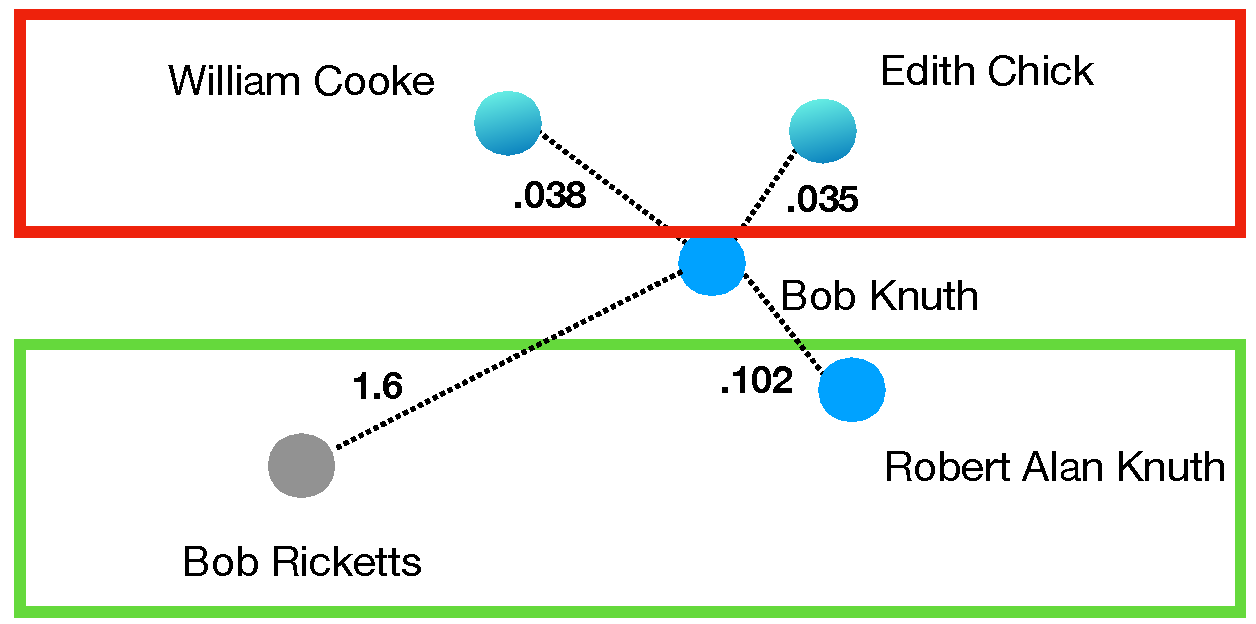
\includegraphics[width=1\linewidth]{word_in_common}
\caption{The model preformed well on somewhat similar names and badly on completely different names}
\label{comp_dif_fail}
\end{figure}
\begin{figure}
\centering
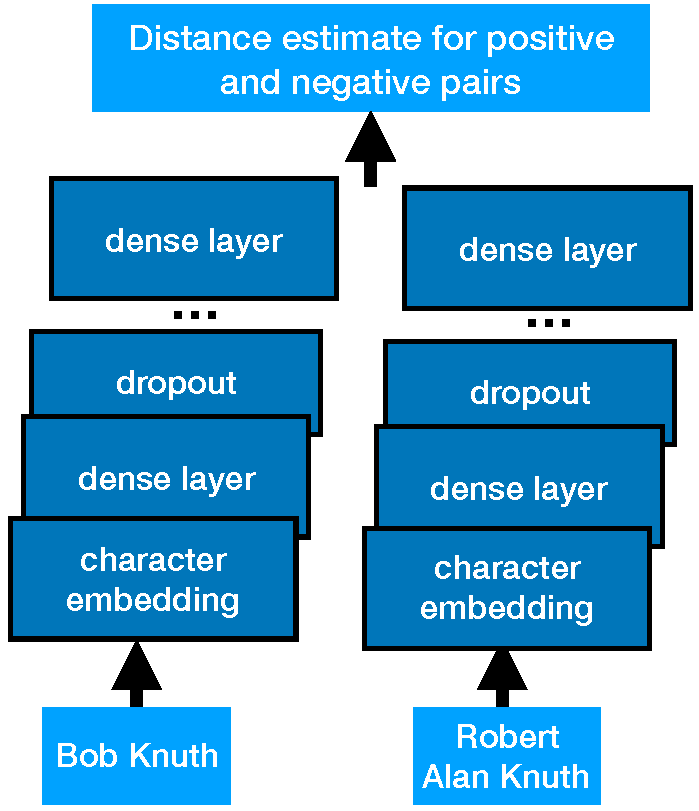
\includegraphics[width=0.5\linewidth]{siamese_arc}
\caption{A siamese network has two networks which share weights which feed into a distance estimator}
\label{siamese}
\end{figure}

\subsection{Approximate Nearest Neighbors}
We used the ANNOY package to find the nearest neighbors in output of the hidden layer computed in the previous section.\cite{annoy_impl} This package approximates the nearest neighbors by first calculating binary trees using the randomized k-d forest method.\cite{ann_paper} These trees are calculated by splitting the vector space by drawing random hyperplanes. Each side of the hyperplane is one node of the binary tree. The algorithm then continues to split each subspace recursively until no more than a predetermined number of items are in each subsection. Some of the neighbors can be found by looking at the items in the same subspace, or subspaces near the target item in the tree. The processes of building a tree is repeated a number of times. By taking a union of the points from all the trees, a reasonable neighborhood is approximated. Once we have a neighborhood of points, we can calculate distance and sort the subset of points. Since much of the time goes into creating the trees, queries can be executed quickly, in logarithmic time.

\subsection{Triplet Loss}
While the previos aproach maps 2 entities at a time using 2 networks that share weights, this aproach maps 3 entities at a time with 3 networks: the anchor the positive and the negative. The loss function minimizes the difference between the anchor and the positive at the same time as it maximises the difference between the anchor and the negative. By doing this we can deal with an unmatched pair and a matched pair at the same time: the anchor is one name, the positive is a match for that name and the negative is another name which is not a match.\cite{schroff2015facenet} We accomplish this by minimizing the following loss function: \[ L(\vec{X}_a, \vec{X}_n, \vec{X}_p) = |\:||\vec{X}_a - \vec{X}_p||^2 - ||\vec{X}_a - \vec{X}_n||^2 + \alpha|\] where $\vec{X}_a$, $\vec{X}_n$, $\vec{X}_p$ are the embedded anchor, negative and positive vectors and $\alpha$ is a constant margin. The key choice here is which vectors to include in the training set. If too many easy triplets are including it will slow down the learning since the constraint will be easily satisfied. If too many hard triplets are included the network will learn a strange function based on unusual cases 

\subsection{LSTM}
A regular Deep Neural network would treat the name like a bag of words, without accounting for order. We experimented with using an LSTM architecture to account for order the words apear in. This makes sense for our use case since first name and last names are different from eachother. In the implimentation we used GRUs (Gated Recurrent Unit), which function like LSTMs but are computationally cheaper.
\section{Experiments}
\subsection{Rule Based}
To test the rule based matcher we ran the blocker followed by the matcher and calculated F-scores based on how many correct matches were in the top 3. We got an F-score of 0.6. Since the issue is mostly false negatives, and therefore even some of the first three slots were often empty, so even if we accept any of the top 1000 as a success, we get an F-score of 0.63, not much better.
\subsection{Siamese Network}
Our first experiment was using a Siamese network to match already blocked entities. The architecture of the network was as shown in Figure \ref{siamese}. As described above this involves two networks that share weights mapping the inputs onto a vector space and computing distance. Before feeding the entities into the networks, we used Kazuma character embeddings to encode each entity as a vector. We used character level embeddings since many names would not have been represented at all if we had used word level embeddings. We then trained the network on our 182772 pairs of names pulled from DBpedia. These are the pairs we have after running the data through the cleanser. We used 95\% of them for training and withheld 5\% for testing. In addition to these pairs we created an equal number of negative pairs to train the model. Wherever possible, the negative pairs had at least one word in common with each other. This was done so that the model would not just learn the obvious function of reject unrelated pairs. We trained the model in 10 epochs. We found that the fscore on the training data was .89 on the test data. This showed that this architecture is an effective matcher. However we only successfully included the correct match in around 15\% of pairs in the top five. This was barely better than the 5\% we got from the embedding alone.
\subsection{Triplet Loss}
The triplet loss experiment was extremely similar to the Siamese one, only we used the Triplet loss network instead of the Siamese one. We used a margin of 1. We also used a GRU instead of a regular deep neural network to capture the order of the words. The last change we used was in selection of negative points, instead of picking them based on some rule, we picked the closest 40 points that were not matches from the character embedding. We did this since those names are the hardest ones for the model to learn, this also avoids the problem in Figure \ref{comp_dif_fail}. When we did this we got 69\% of the items in the top 40. This is a relatively effective blocker. It also correctly placed 97\% of positives closer to the anchor than negatives, making it a very effective matcher.
\section{Conclusions}
While we have a very good machine learning based matcher, that does not appear to translate into very good blocking. We still need to explore why we only getting around 69\% of the matches in the top 40 items, when we have the positive closer than the negative in 97\% of cases.  
%\end{document}  % This is where a 'short' article might terminate

% ensure same length columns on last page (might need two sub-sequent latex runs)
\balance

%ACKNOWLEDGMENTS are optional

% The following two commands are all you need in the
% initial runs of your .tex file to
% produce the bibliography for the citations in your paper.
\bibliographystyle{abbrv}
\bibliography{paper}  % vldb_sample.bib is the name of the Bibliography in this case
% You must have a proper ".bib" file
%  and remember to run:
% latex bibtex latex latex
% to resolve all references

% ****************** APPENDIX **************************************

% Example of an appendix; typically would start on a new page
%pagebreak


\end{document}
